\documentclass{l4proj}

\usepackage{url}
\usepackage{fancyvrb}
\usepackage{amsmath}
\usepackage{amsthm}
\usepackage[final]{pdfpages}
\usepackage{hyperref}
\usepackage[utf8]{inputenc}
\usepackage{listings}
\usepackage[toc]{glossaries}
\usepackage[style=authoryear, backend=biber]{biblatex}
\usepackage{graphicx}

\addbibresource{l4proj.bib}
\makeglossaries
\glstoctrue


% GLOSSARY =====================================================================

\newglossaryentry{homozygous}{
  name=homozygous,
  description={A homozygous individual possesses two identical alleles of a gene, either both encoding a given trait or the lack of it. A homozygous individual without a given trait is called homozygous recessive for that trait. A homozygous individual with a given trait is called homozygous dominant}
}

\newglossaryentry{selective sweep}{
  name=selective sweep,
  description={When natural selection exerts positive or negative selective pressure on individuals possessing a given trait the alleles encoding this trait will respectively dominate the population or disappear from the population. The process is referred to as selective sweep.}
}

\newglossaryentry{heterozygous}{
  name=heterozygous,
  description={A heterozygous individual possess two different alleles of a gene, one of which encodes a given trait, and one of which encodes a lack of the trait}
}

\newglossaryentry{dominant}{
  name=dominant,
  description={A dominant inheritance scheme is a scheme in which individuals possessing one or two copies of a gene encoding the trait exhibit the trait. An individual can be called homozygous dominant for a trait if it is homozygous and possesses the trait}
}

\newglossaryentry{MRCA}{
  name=MRCA,
  description={An MRCA of a generation at time $t$ is a common ancestor which is the most recent, i.e. precedes the population by the least number of generations.}
}

\newglossaryentry{recessive}{
  name=recessive,
  description={The recessive inheritance scheme is a scheme in which only individuals possessing two copies of a gene encoding the trait exhibit the trait. An individual can be called homozygous dominant for a trait if it is homozygous and it does not possess the trait}
}


\newglossaryentry{autosomal}{
  name=autosomal,
  description={An autosomal gene is located on one of the numbered chromosomes (as opposed to the sex chromosomes). Organisms typically have a pair of autosomal chromosomes, one from the mother and one from the father}
}

\newglossaryentry{polyploid}{
  name=polyploid,
  description={Most organisms have only two versions of each autosomal gene. Some organisms have 4, 6, 8 or more copies of each gene. Such organisms are called polyploid organisms}
}

\newglossaryentry{chromosome}{
  name=chromosome,
  description={chromosome is a collections of genes. Organisms usually have several chromosomes, usually classified into numbered chromosmes, which host autosomal genes, and sex chromosomes, which host sex-linked genes}
}


\newglossaryentry{sex-linked}{
  name=sex-linked,
  description={A sex-linked gene is located on one of the sex chromosomes (as opposed to one of the numbered chromosomes). Organisms usually have either one or two copies of sex-linked genes, depending on sex}
}

\newglossaryentry{allele}{
  name=allele,
  description={A version of a gene. Each gene can have one or multiple alleles. Existence of many gene versions is the reason for variety within population. Some alleles can corrupt normal body function and result in disease}
}

\newglossaryentry{population graph}{
  name=population graph,
  description={A population graph $G_{p} = (V, E)$ is a Directed Acyclic Graph, where $V$ is the set of all simulated individuals, dead or alive, and $E$ is a collection of all pairs of sims $(u, v)$ such that $u$ is a parent of $v$}
}

\newglossaryentry{locus}{
  name=locus,
  plural={loci},
  description={A placeholder for a gene. Locus is situated on a chromosome and can hold a version of the gene -- see \gls{allele}. If the locus is situated on one of the numbered chromosomes, the gene is called \gls{autosomal}. If the gene is on one of the sex chromosomes, the gene is called \gls{sex-linked}}
}



\newtheorem*{quest}{Research Question}
\newtheorem{assum}{Assumption}
\newcommand{\Tmrca}{T\raisebox{-.4ex}{\scriptsize MRCA}}
\newcommand{\genotype}[2]{\ensuremath{(\mathrm{#1}, \mathrm{#2})}}

\renewcommand*{\glstextformat}{\textbf}

\newif\ifdebug

\debugfalse

\lstset{basicstyle=\ttfamily\footnotesize,breaklines=true}

\begin{document}


\title{The effect of natural selection on relatedness in randomly mating population}
\author{Adam Kurkiewicz}
\date{March 25, 2016}
\maketitle

% ABSTRACT =====================================================================

\begin{abstract}

A flexible population simulation framework is designed and implemented in Python. The framework allows to simulate biological populations, whose evolution is specified by the user, through implementing python functions defining desired breeding, mating, mutation, migration and inheritance schemes. The effect of running each simulation is a file containing a complete information on the entire history of the population, including genotypes of all simulated individuals, parent-child relationships, the generation number each sim belonged to when alive, and the location it occupied. Produced population file can be processed algorithmically and statistically to investigate the simulated population. An experiment is designed in order to answer the research question: Does natural selection affect relatedness in a species? While we fail to reach a definite conclusion using the methods employed, the areas for further investigation are proposed.

\end{abstract}

\educationalconsent

\tableofcontents

% INTRODUCTION =================================================================

\chapter{Introduction}
\label{intro}

\ifdebug
  Introduction. This should place the work in context and will be developed from the introduction produced for assessment.
\fi

\pagenumbering{arabic}

\section{Context of the work}

The publication of ``On the Origin of Species'' \parencite{darwin59} is generally accepted to be a founding stone of still vigorously researched field of evolutionary biology. Over the years, as the understanding of the field deepened, it became clear that certain scientific questions within the field can only be answered by obtaining progress in related fields, like establishing laws governing inheritance (genetics) \parencite{mendel}, understanding the role of organic molecules in the process of inheritance (molecular biology) \parencite{watson53}, understanding population dynamics of predator-prey system using both continuous and discrete methods (mathematical biology), understanding the character of population variability at molecular level (neutral theory of molecular evolution, Markov processes) \parencite{kimura68, dayhoff73}, studying of historical populations (archaeology, anthropology, linguistics) \parencite{dubois}, proposing and verifying hypotheses about populations based on quantitative evidence (statistics) \parencite{bronzeAgeEurasia}, modeling and simulating biological systems \textit{in silico} (systems biology), and many others.

While the research presented in this work falls within the realm of computational biology, when referring to other, connected fields we might occasionally need specialized jargon. A glossary of technical terms in use is included at the end of this work. Throughout the text words and phrases in bold (e.g. \gls{autosomal}) are explained in the glossary.

\section{Research question}\label{TMRCA}
The scientific question that we will try to answer in this piece of work is directly connected with evolution by natural selection and perhaps might have even occurred to Darwin himself:

\begin{quest}
Does natural selection affect relatedness in a species? Are individuals in a species under selective pressure more likely to be closely related?
\end{quest}

We will seek to answer this question using a computer simulation. First, we have to decide on how to measure relatedness. We will follow \cite{rohde04} and focus on computing time (in generations) that is taken for a group of simulated individuals to reach a Most Recent Common Ancestor (MRCA). More precisely, we will speak of a \gls{population graph}, which we will define to be a Directed Acyclic Graph (DAG), with vertices representing all individuals ever alive and directed edges representing the parent-child relationship between individuals. Additionally, each vertex will be labeled with complete information on individual's traits. For any point in time all individuals capable of inter-breeding at that point will be referred to as ``generation at time $t$'', or simply ``generation'', if the time can be inferred from the context. An MRCA of a generation at time $t$ will be a common ancestor which is the most recent, i.e. precedes the population by the least number of generations. The time (in generations) that is taken to reach such individual will be denoted by $T_{MRCA}$.

There are other, auxiliary questions we will have to answer on our way. Most crucially we will have to decide on such important details of our simulation as the mating scheme, migration, competition for resource, survivability, number of offspring, etc. Often we will be able to use the choices of parameters already made by others, e.g. breeding scheme \parencite{peng10}. We prepare the ground in chapter \ref{review}. Appropriate methodology is decided upon in chapter \ref{methodology}. We discuss the architecture of the computer program which constitutes the solution, and is on its own a valuable contribution to the field, in chapter \ref{practical}. The experiment, which constitutes a novel contribution to the field is discussed in chapter \ref{research}. The conclusions will be drawn in chapter \ref{conclusion}. The source code of all developed computer programs can be accessed on github \parencite{Kurkiewicz16} 

% REVIEW OF THE FIELD ==========================================================

\chapter{Review of the field}\label{review}

\section{Basic inheritance}

Presented work is by no means the first attempt at quantitative study of population genetics. What follows is a review of the most relevant achievements in the field.

\subsection{Early days}
Ever since three European scientist simultaneously and independently rediscovered \& experimentally confirmed Gregor Mendel's theory of inheritance [find the original works of DeVries, Correns and Tscherma, Roberts, H. F. Plant Hybridization before Mendel. Princeton: Princeton University Press, 1929.], the interplay between Mendelian Inheritance and Darwinian Evolution has been hotly debated. One claim popular at the time has fallaciously asserted that Mendelian Genetics cannot be a correct model of trait inheritance [cite this guy whose name starts with U]. The reasoning at the core of the claim was that dominant alleles over time sweep the entire population, thus eliminating variation within the population, rendering evolution by natural selection impossible. This misconception was debunked in a very short letter to the editor of ``Science'' by a famous English number theorist \parencite{hardy08}. The letter is a truly master example of a presentation of non-trivial mathematical thought in a manner both rigorous and understandable, even to non-experts. Let us recall Mendel's laws of inheritance before we present Hardy's argument.

\subsection{Mendelian Inheritance}

Let us start by briefly sketching a relevant subset of the laws of Mendelian Inheritance. A more comprehensive reference can be found in an annotated English translation of the original work of Mendel by \cite{mendel}.

Firstly, we will be acting under the assumption that each animal characteristic (trait) is either present, or not present in a given organism because of:
\begin{assum}\label{genotypes}
  possession by this organism of one, two or none copies of a gene encoding this characteristic.
\end{assum}

\begin{assum}\label{dominance}
  the mode of expression of the characteristic, which can be either \gls{dominant} or \gls{recessive}.
\end{assum}

We have to remark that these assumptions may not be obviously true for certain seemingly continuous, partially environment-dependent characteristics such as height, weight or individual's position in the autism spectrum. However experiments using various methods have consistently asserted that ~80\% of human height is inheritable \parencite{heightTwins, heightJustSiblings}. Although the challenge of identifying all genes affecting height is still open, recent progress using a cross-discipline technique called Genome Wide Association Study (GWAS) identified over 40 genes, which contribute 5 percent points towards total height heritability. To play devil's advocate further, it has been recently established that important traits can be acquired and inherited by non-genetic means in both plants \parencite{palmOilKernel}, non-human animals \parencite{dolinoy_maternal_2007} and humans \parencite{yehuda_holocaust_2015}, giving rise to the field of Epigenetics. We shall consider both environmental and epigenetic factors to be outside of the scope of this research. A curious reader is referred to an accessible, popular science discussion of the topic of GWAS, height inheritance and epigenetics by \textcite{GWASDiscussion}. A concerned reader should find assurance in that a great many traits do obey Mendelian's Inheritance straightforwardly. A comprehensive database for human traits, maintained by John Hopkins University at omim.org \parencite{omim16}, finds 24617 such genes using the match-all wildcard $*$, including 22044 \gls{autosomal} genes (as of \date{March 13, 2016}).

Before we proceed let us recall the following, standard notation: if an \gls{allele} encoding a trait is determined to be \gls{dominant} we will represent it with capital letter, e.g. $\mathrm{A}$. In such case a lack of trait will be considered \gls{recessive} and be denoted as $\mathrm{a}$. Under the assumption \ref{genotypes}, we will consider all three possible genotypes: \genotype{A}{A} -- homozygous dominant, \genotype{A}{a} -- heterozygous and \genotype{a}{a} -- homozygous recessive. Of these the first two the genotypes \genotype{A}{A} and \genotype{A}{a} will result in an individual possessing the characteristic. An individual with the last genotype \genotype{a}{a} will not exhibit the trait. Analogously, one can consider a trait inherited recessively, and in such case the above description is true when ``trait'' is mutually exchanged with ``lack of trait'', ``not exhibit the trait'' with ``exhibit the trait'', etc.

Further, we will assume that
\begin{assum}\label{offspring}
  in offspring each of the two alleles present comes from the parents, precisely one from the mother and one from the father. Each of the parent's two alleles has a 50\% chance of being inherited.
\end{assum}
We can use our assumptions \ref{genotypes}, \ref{dominance}, \ref{offspring} to work out that in a specific case of breeding two heterozygous individuals, an \genotype{A}{a} mother and an \genotype{A}{a} father, each individual offspring will have either of 3 possible genotypes with probabilities $\frac{1}{4}$ for \genotype{A}{A}, $\frac{1}{2}$ for \genotype{A}{a} and $\frac{1}{4}$ for \genotype{a}{a}. Table \ref{offspringTable} gives all possible outcomes of breeding all possible genotypes involving one characteristic along with corresponding probabilities. If the desired mode of inheritance is dominant, the reader can interpret \genotype{A}{a} and \genotype{A}{A} as trait-positive and \genotype{a}{a} as trait-negative. For the recessive case, \genotype{a}{a} is trait-positive and both \genotype{A}{A} and \genotype{A}{a} are trait-negative.

\begin{table}[]
    \centering
    \begin{tabular}{cc||c|c|c|}
    \cline{3-5}
     &  & \multicolumn{3}{c|}{mother} \\ \cline{3-5} 
     &  & \genotype{a}{a} & \genotype{A}{a} & \genotype{A}{A} \\ \hline\hline
    \multicolumn{1}{|c|}{father} & \genotype{a}{a} & \genotype{a}{a} 1 & \begin{tabular}[c]{@{}l@{}}\genotype{a}{a} $\frac{1}{2}$ \\ \genotype{A}{a} $\frac{1}{2}$ \end{tabular} & \genotype{A}{a} 1 \\ \cline{2-5} 
    \multicolumn{1}{|l|}{} & \genotype{A}{a} & \begin{tabular}[c]{@{}l@{}}\genotype{a}{a} $\frac{1}{2}$\\ \genotype{A}{a} $\frac{1}{2}$\end{tabular} & \begin{tabular}[c]{@{}l@{}}\genotype{a}{a} $\frac{1}{4}$\\ \genotype{A}{a} $\frac{1}{2}$\\ \genotype{A}{A} $\frac{1}{4}$\end{tabular} & \begin{tabular}[c]{@{}l@{}}\genotype{A}{a} $\frac{1}{2}$\\ \genotype{A}{A} $\frac{1}{2}$\end{tabular} \\ \cline{2-5} 
    \multicolumn{1}{|l|}{} & \genotype{A}{A} & \genotype{A}{a} 1 & \begin{tabular}[c]{@{}l@{}}\genotype{A}{a} $\frac{1}{2}$\\ \genotype{A}{A} $\frac{1}{2}$\end{tabular} & \genotype{A}{A} 1 \\ \hline
    \end{tabular}
    \caption{Possible offspring genotypes with corresponding probabilities}
    \label{offspringTable}
\end{table}

Finally, we have to remark that the assumption \ref{offspring} may not be correct in rare cases of \gls{sex-linked} characteristics (e.g. colour-blindess). This research will focus exclusively on \gls{autosomal} genes.

\subsection{Hardy-Weinberg equilibrium.}

\begin{samepage}
Let us desribe a distribution of genotypes in the population as the ratio of dominant homozygotes to heterozygotes to recessive homozygotes, symbolically $$p:2q:r$$ $2q$ appears in the ratio to ease the computation.
\end{samepage}

The ingenious insight of \cite{hardy08} is in observing that for certain values of $p$, $q$ and $r$, the ratio will stay unchanged from generation to generation; ratios with this property he calls ``stable''. Hardy gives conditions for stability, and shows that ratios that aren't stable converge to ``stable'' ratios as the population develops. Hardy's argument is based on assuming an arbitrary ratio in the parent generation and computing the ratio of the children's generation. He accomplishes that using a table much like \ref{offspringTable}, and then solving a system of three degree-2 polynomials in three indeterminates: $p$, $q$ and $r$. The result, $q^{2}=pr$, is a necessary and sufficient condition for the ratio to be stable. We have to remark a few assumptions made by Hardy for his proof of the stability condition. Namely, the population is assumed to be isolated, randomly mating, it is assumed to be large, and the number of men and women is assumed to be equal. Hardy's argument does not take into account natural selection.

\section{Work of Fisher}

The work of Ronald Fisher had drastic influence on the landcape of both statistics and population genetics. Apart from introducing influential statistical terminology (such as the concept of variance, defined as standard deviation squared, \cite{Fisher18}), Fisher gave modern shape to the notion of null hypothesis testing. He also invented a range of statistical methods, such as one-way analysis of variance (ANOVA). On the biological side, Fisher was behind the realisation that sexual selection is comparatively stronger, and more consistent than natural selection. He formulated the concept of Fisherian runaway and proposed the sexy sons hypothesis. He also proposed the mechanism for inheritance of complex traits \parencite{Fisher18}.  His work on coalescent processes gave rise to the coalescent method, which is of interest for the project, as it could be potentially used to answer the research question.

\section{Coalescent method}

The coalescent method, in its most basic form, is used to predict the time (in generations) one has to go back in the population graph for any genetic trait to reach the individual it originated from (``coalesce''). The method is usually employed for a group of individuals with unknown predecessor structure, which makes it suitable for use in situations when data regarding only extant individuals is available. Given an extant population, the coalescent method works backwards in time, with generations in hypothetical ancestry assigned probabilities of containing the coalescent. Although in this basic application the coalescent method is relatively straightforward to apply, once natural selection is included the method gets subtle and very complicated, with most research still open-ended \parencite{Wakeley16}. For a comprehensive review, a reader is referred to \cite{Wakeley16}. 

\section{Forward-Time Modeling}

Finally, let us move on to the most recent population modeling method, so called forward-time modeling. While the idea of running a forward-time population model is relatively straightforward, it has long been assumed that its value is only educational \parencite{peng05}. However, with the advent of vast computational power, and a desire to model complex populations, the forward-time modeling has steadily gained popularity. Genetic Simulation Resources lists 54 publications \parencite{GSR16}, which have utilised just a single forward-time simulation framework simuPOP \parencite{peng05}.

Forward-Time Modeling is based on the idea of assuming an initial population (generation 0) and rules governing that population's development in time. Each subsequent generation is obtained by applying these rules to the previous generation. The rules are usually probabilistic, and randomness is obtained from pseudo-random number generators, like Mersenne Twister \parencite{Matsumoto98}. This work is extensively based on two particular models, and can be perhaps viewed as an attempt at merging the two approaches. The first model due to \cite{rohde04} looks at the relatedness of the simulated population through computing how far back in time one has to go to find the \gls{MRCA} of the final generation in the simulation. Some detail on their approach is given in the next section. The second model due to \cite{peng10} looks at modeling a population undergoing a \gls{selective sweep} of various strength for the purpose of simulating GWAS data. This model in turn is not concerned with computing MRCA. A model very similar to this second model is described in detail in chapter \ref{research}.

\section{Modelling the recent common ancestry of all living humans}

A research of \cite{rohde04} is a very successful blend of statistical theory and forward-time modeling applied in the context of human population from 20000 BC until the modern day. The purpose of the simulation is to compute the most recent common ancestor of present-day human population. The authors use historical and anthropological data, and an occasional educated guess, to model the spread of humans out of Africa, using a town-country-continent model, with random mating at town level, migration between towns, between countries and between continents. The authors keep the migration rate ``conservatively low'', as they are trying to avoid underestimating $T_{MRCA}$, and in accordance with their theoretical investigation the migration rate and $T_{MRCA}$ are inversely proportional.

The authors decide to use a continuous-generation model, with individuals born throughout the lives of their parents (as opposed to at the end of their life, as with discrete generation model), co-inhabiting and perhaps even mating across generations. The authors use their model to predict that $T_{MRCA}$ of present humans is approximately 100 generations, which is not very far from a theoretical number of about 30 under an unrealistic assumption of random mating.

The model proposed by the authors does not take into account natural selection.

% METHODOLOGY =====================================================

\chapter{Choice of methodology}\label{methodology}

After a consideration given to both coalescent and forward-time approach, the forward time approach is chosen for the following reasons:

\begin{itemize}
\item As argued by \cite{peng10}, forward-time modeling is particularly well-suited for modeling populations under selective pressure.
\item Writing computer code is at heart of forward-time modeling, as the technique is fundamentally computational. There are challenges involving code correctness, performance and choice of algorithms. Handling these appropriately can be considered a good challenge for a computer programmer.  
\item Coalescent method, with its statistical difficulties could be cognitively prohibitive, especially taken into account the amount of time that could be spent on the project and the skill-set of the investigator.  
\end{itemize}

The approach was split into two units of work. The first was the design and implementation of a forward-time modeling framework, suitable for our purpose. The framework is implemented as a python module, and was accomplished to strict software engineering standards, is implemented in a portable way, thoroughly tested, reasonably documented, and easily extensible. The second unit of work was the design and execution of the experiment itself.

We report on both in chapters \ref{practical} and \ref{research}.


% REPORT OF PRACTICAL WORK =====================================================

\chapter{Report of practical work}\label{practical}

\section{Natural Selection Framework}
An important contribution of this research work is an implementation of a forward-time population modeling framework. The framework is then used to investigate the research question that we're interested in by focusing on particular population models of our interest. However, the framework does not force its users into any particular choice of the model. A wide range of real-life populations can be modeled by implementing appropriate mutation, breeding, mating, natural selection, migration and inheritance schemes. The schemes are implemented as python functions, and can be glued together using the framework's API into a full population model. This approach is not dissimilar from simuPOP \parencite{peng05}, a particularly successful forward-time simulation framework, which has been used extensively to model populations under selective pressure, for example to model population divergence due to local adaptation \parencite{naturalSelectionSignatures16}. Let us discuss the design of the framework focusing on similarities and differences with simuPOP.

\subsection{High-Level overview}
The central unit of any simulation in the framework is a ``sim''. Sims are computational abstractions of biological individuals. Sims are assigned partners in accordance with a mating scheme, can sexually reproduce with other sims of opposite sex, and produce offspring in accordance with a breeding scheme. Both mating and breeding schemes can be chosen from any provided by the framework or be user-defined. Some mating and breeding schemes are capable of taking into account the individual's relative fitness and therefore can be used to get insights into the process of natural selection. Sims live on the surface of a unit sphere. Each sim after birth is assigned the position of its female parent. After birth and before mating and breeding each sim migrates in accordance with a specified migration scheme. Each sim possess a genome, which is an encoding of that sim's genes.

The set of all sims in the simulation forms the set of vertices $V$ in the \gls{population graph} $G_{p} = (V, E)$. A pair of sims $(u, v)$ belongs to the set of edges $E$ of $G_{p}$ if the sim $u$ is a parent of the sim $v$. It is easily noticed that $G_{p}$ is a DAG, as no sim can be its own ancestor. We call sims capable of interbreeding at time $t$ to be a generation. Like in simuPOP, the framework is designed in such way that generations are discrete, i.e. all sims in the parent generation die before any sims in the children generation are capable of reproduction. This simplifies the construction of the framework.

Finally sims are serialised into json format and output to hard drive for further analysis. The analysis stage consists of computing MRCA of each generation of sims in the population graph.

simuPOP provides most of the same functionality, however there are significant differences between the two programs. Exact comparison is difficult, because simuPOP is mature software in constant development for over a decade, whereas the proposed framework is an effect of 7 months of part-time development.

Most notably, simuPOP does not allow for graph-theoretic analysis of simulated populations, and does not support outputting population graphs into permanent storage for later analysis. Aside from the educational aspect of creating my own framework this was the main reason why the effort was undertaken.

\subsection{Performance and porability}

SimuPOP achieves low memory and CPU footprint by using python's \textit{extension modules}, which allow more direct access to underlying hardware than pure python. However, there are significant drawbacks of using \textit{extension modules}.

Firstly, development is slowed down by higher cognitive burden put on the programmer, as \textit{extension modules} are typically written in C++, which is arguably less user-friendly than pure python. The following snippet of simuPOP's source code serves as good example:

\begin{lstlisting}
PyObject * genoObj = PyTuple_New(alleles.size());
// set value
for (size_t j = 0; j < alleles.size(); ++j)
    PyTuple_SET_ITEM(genoObj, j, PyInt_FromLong(alleles[j]));
return genoObj;
\end{lstlisting}

which could be equivalently expressed in pure python 

\begin{lstlisting}
genoObj = tuple(alleles)
return genoObj    
\end{lstlisting}

Secondly, the use of extension modules limits execution environment of simuPOP to CPython, whereas the framework proposed has been successfully tested both under CPython 2 and 3 (the entire framework), pypi and jython (with exception of the graph analysis module). Using pure python therefore results in much higher portability.

Let us end this note on performance by saying that the performance of the framework is satisfactory for our purpose. Timing one of the simulation scripts (with MRCA analysis) reveals that the simulation of an initial population of 1000 sims for 70 generations accomplishes in under 2 minutes on consumer grade hardware.

\subsection{Genome}
SimuPOP allows for extensive modeling of genomes, such as modeling multiple loci situated on multiple \gls{chromosome}s, even in \gls{polyploid} organisms \parencite{simuPOP16}.

The proposed framework takes much simpler approach consistent with our requirement of investigating a single feature, in its present form allowing for only one \gls{locus} capable of containing only 2 alleles.

\subsection{Migration}
The proposed framework takes a different approach to modeling migration than either simuPOP or \cite{rohde04}. Both simuPOP and the other program allow for maintaining partial population substructure through simulating many small randomly breeding sub-populations with limited migration between these sub-populations. The proposed framework is different in that it allows for continuous diffusion of sims on the surface of the world they live in, which is a unit sphere. Appropriate spherical trigonometry was derived using a blend of traditional paper-based computation and Sage \parencite{sage14}. The README.md file accompanying the source gives sufficient description to reproduce these results.

The sims can migrate on the surface of the sphere using two different schemes, the wanderer scheme, which positions any sim in a random (pole-adjusted) point on the sphere, and homebody, which moves a sim by at most a great-arc distance k on the sphere, in a random direction. Additional types of migrators can be implemented by the user.

\subsection{Mutations and Inheritance}

The framework allows for a simulation of \gls{autosomal} recessive and \gls{autosomal} dominant alleles. The \gls{sex-linked} genes are not supported, unlike in simuPOP.

\subsection{Natural Selection}

The frameork implements the natural selection scheme proposed by \cite{peng10}, and discussed in detail in chapter \ref{research}. The user can easily define any other natural selection scheme.

\subsection{Generations}
discrete generations as in simuPOP. This is unlike Rohde and Olhsen.

\subsection{Mating and Breeding}
Depending on 
capture difficulty in random mating -> random fluctuations in population

\subsection{Code Correctness}
Great care was taken to ensure correctness. As of the project submission no discovered bugs or outstanding issues remain, and extensive unit testing has been in place throughout the project. The framework consists of about 1600 lines of code and contains 25 test cases, which provide about 75\% test coverage. The most challenging module, ``processGraph.py'' is most extensively tested, with 10 test cases and 97\% test coverage.

An interesting way of testing the framework was devised to solve the issue of inherent lack of determinism in test case resuls. As simulated processes are probabilistic in nature, a traditional way of testing the program through an instance of input for which output is known could not be realised. Instead, whenever possible, theoretical consideration of the expected distribution of output was undertaken, and a range of values was chosen as valid. The range was chosen in such way as to make it incredibly unlikely for the test case to fail. For binomial distribution for example, 5 standard deviations around mean were taken to form the range.

\subsection{Extensibility}

A major change to the library occurred between revisions eadc6756 and 1af29cde. The change was due to a realisation that a particular algorithm chosen to compute MRCA was performing poorly, and the implementation of an alternative algorithm was undertaken. This required several changes across two modules, the module responsible for graph generation and the module responsible for graph processing. The change was accomplished in a few days of work, and the difficulties rather than in code integration lied in it's high cognitive load. Presumably the change would be more difficult if the safety net of extensive test coverage was not present.  

\subsection{Documentation}
A reasonable part of the framework is documented and is made available through pydoc (and pydoc3). An instruction on how to access the manual is given in detail in the project's README.md, which accompanies the source code. The source code can be accessed on github \parencite{Kurkiewicz16}


% REPORT OF RESEARCH WORK ======================================================

\chapter{Report of research work}\label{research}
This should bring out the insights and new ideas produced by the review and may continue to suggest further practical work, which would test these ideas. Most importantly, the report should clearly state the overall value of the work which has been done - this should not be lost in a welter of detail.

\section{Selective Sweep in Randomly Mating Population}

An experiment was carried out in order to quantify the effect of positive selection on relatedness in a small, randomly mating population. The relatedness was measured using $T_{MRCA}$ (as discussed in chapter \ref{intro}) of a carefully selected generation in this population.

Throughout the experiment randomness was obtained from python's default random module, which implements Mersenne Twister, a good choice of pseudo-randomness for scientific simulations \parencite{Matsumoto98}. Let us explain the experiment's design.

The initial simulation size was set to be 100 sims, of random sex, and uniformly distributed on the unit sphere. One of the sims, chosen at random, was assigned a \gls{heterozygous} genotype. All other sims were assigned \gls{homozygous} recessive genotypes. The chosen mode of gene expression was \gls{dominant}. The presence of a trait in an invidual would give that individual a comparative breeding advantage of 5\% over an individual without the trait. Each subsequent generation of the simulation was obtained as follows. For each sim in the next generation, first parent was chosen at random from the previous generation. The probability of any sim $s$ being chosen as the first parent can be expressed by a formula
$$p(s, S) = \frac{f(s)}{\sum_{s' \in S}^{}f(s')}$$
where $S$ is the set of all sims in the previous generation (including $s$), and $f(s)$, the sim's absolute fitness, is defined by

$$
f(s) = \begin{cases}
  1.05 \text{, if sim $s$ has the trait} \\
  1 \text{, if sim $s$ does not have the trait} \\
\end{cases}
$$

The second parent was chosen to be the closest sim of opposite sex (as measured by the great circle distance on the unit sphere). The number of sims in the next generation was adjusted to be equal to the number of sims in the previous generation. After birth and before mating each sim migrated to a randomly chosen place on the unit sphere. This model closely follows the one described by \cite{peng10}. It differs from the model of \cite{rohde04} by usage of discrete generations (the previous generation dies before the next generation can breed) as opposed to continuous real-life like generations.

The simulation was run until the trait had spread to the entire population or the trait died out. In the former case, the simulation was included in the sample, in the latter case the simulation was discarded. It is worth pointing out that the length of each simulation measured by generations was variable, i.e. it did not always take the same number of generations for a simulation to reach full trait saturation.

The investigated sample consisted of 200 simulation runs of the experiment described above. For each simulation in this sample, a control simulation was generated with the relative advantage of possessing the trait removed (all sims equally likely to become the first parent) and the length in generations equal to that of the corresponding observation from the sample. This had given a control sample of 200 sims.

Both the investigated and the control sample were processed in the following way: for each simulation in either sample a generation exactly in the middle of the simulation (rounded down if the number of generations happened to be odd) was chosen, and $T_{MRCA}$ was computed for this generation.

This had resulted in two samples of 200 non-negative integers each. The table \ref{populationTable} gives some common statistics for these numbers. Looking at the table we can infer that both the sample and the control are actually collections of integers in the interval $[5, 7]$. We expect a lot of repetitions.

\begin{table}[]
    \centering
    \begin{tabular}{|c|c|c|}
    \hline
     & sample & control \\ \hline\hline
     average & 6.415 & 6.37 \\ \hline
     median & 6 & 6 \\ \hline
     mode & 7 & 7 \\ \hline
     min & 5 & 5 \\ \hline
     max & 7 & 7 \\ \hline
    \end{tabular}
    \caption{statistics for population of size 100 and relative advantage 1.05}
    \label{populationTable}
\end{table}

The null hypothesis was chosen so that both the investigated sample and the control sample $T_{MRCA}$s come from the same distribution. This hypothesis was tested using Mann-Whitney U-test (ties adjusted and continuity corrected) and Kolomogorov-Smirnov (without continuity correction) two sample test. In Table \ref{nullHypothesisTable} we report the p-values.

\begin{table}[]
    \centering
    \begin{tabular}{|c|c|c|}
    \hline
    & Mann-Whitney & Kolomogorov-Smirnov \\ \hline
    p-values & 0.258987 & 0.999987 \\ \hline
    \end{tabular}
    \caption{p-values of null-hypothesis for population of size 100 and relative advantage 1.05}
    \label{nullHypothesisTable}
\end{table}

Analogous experiments were executed for all combinations of relative advantage in the rage [1.05, 1.10] and population sizes in the range [120, 140, 160, 180, 200]. Resulting 10 statistical tests are reported below. The reader is trusted to apply the Bonferroni correction of 11, when interpreting the p-values.

\begin{table}[]
    \centering
    \begin{tabular}{|c|c|c|}
    \hline
    & Mann-Whitney & Kolomogorov-Smirnov \\ \hline
    p-values & 0.475 & 0.999 \\ \hline
    \end{tabular}
    \caption{p-values of null-hypothesis for population of size 120 and relative advantage 1.10}
\end{table}

\begin{table}[]
    \centering
    \begin{tabular}{|c|c|c|}
    \hline
    & Mann-Whitney & Kolomogorov-Smirnov \\ \hline
    p-values & 0.0962 & 0.981 \\ \hline
    \end{tabular}
    \caption{p-values of null-hypothesis for population of size 140 and relative advantage 1.10}
\end{table}

\begin{table}[]
    \centering
    \begin{tabular}{|c|c|c|}
    \hline
    & Mann-Whitney & Kolomogorov-Smirnov \\ \hline
    p-values & 0.0663 & 0.708 \\ \hline
    \end{tabular}
    \caption{p-values of null-hypothesis for population of size 160 and relative advantage 1.10}
\end{table}

\begin{table}[]
    \centering
    \begin{tabular}{|c|c|c|}
    \hline
    & Mann-Whitney & Kolomogorov-Smirnov \\ \hline
    p-values & 0.0406 & 0.708 \\ \hline
    \end{tabular}
    \caption{p-values of null-hypothesis for population of size 180 and relative advantage 1.10}
\end{table}

\begin{table}[]
    \centering
    \begin{tabular}{|c|c|c|}
    \hline
    & Mann-Whitney & Kolomogorov-Smirnov \\ \hline
    p-values & 0.0859 & 0.674 \\ \hline
    \end{tabular}
    \caption{p-values of null-hypothesis for population of size 200 and relative advantage 1.10}
\end{table}

\begin{table}[]
    \centering
    \begin{tabular}{|c|c|c|}
    \hline
    & Mann-Whitney & Kolomogorov-Smirnov \\ \hline
    p-values & 0.05 & 0.999 \\ \hline
    \end{tabular}
    \caption{p-values of null-hypothesis for population of size 120 and relative advantage 1.05}
\end{table}


\begin{table}[]
    \centering
    \begin{tabular}{|c|c|c|}
    \hline
    & Mann-Whitney & Kolomogorov-Smirnov \\ \hline
    p-values & 0.104 & 0.893 \\ \hline
    \end{tabular}
    \caption{p-values of null-hypothesis for population of size 140 and relative advantage 1.05}
\end{table}


\begin{table}[]
    \centering
    \begin{tabular}{|c|c|c|}
    \hline
    & Mann-Whitney & Kolomogorov-Smirnov \\ \hline
    p-values & 0.244 & 0.999  \\ \hline
    \end{tabular}
    \caption{p-values of null-hypothesis for population of size 160 and relative advantage 1.05}
\end{table}

\begin{table}[]
    \centering
    \begin{tabular}{|c|c|c|}
    \hline
    & Mann-Whitney & Kolomogorov-Smirnov \\ \hline
    p-values & 0.0609 & 0.708  \\ \hline
    \end{tabular}
    \caption{p-values of null-hypothesis for population of size 160 and relative advantage 1.05}
\end{table}


\begin{table}[]
    \centering
    \begin{tabular}{|c|c|c|}
    \hline
    & Mann-Whitney & Kolomogorov-Smirnov \\ \hline
    p-values & 0.0769 & 0.999  \\ \hline
    \end{tabular}
    \caption{p-values of null-hypothesis for population of size 200 and relative advantage 1.05}
\end{table}

% CONCLUSION ===================================================================

\chapter{Conclusion}\label{conclusion}

\section{Inconclusive results}

The experiment carried out did not provide evidence allowing to reject the null hypothesis with the cut-off value of 0.05 (0.0045 after Bonferroni correction), which states that selective sweep has no influence on $T_{MRCA}$. There can be numerous reasons for this outcome. Firstly there might be no influence indeed, or the influence might be so slim, that a very big number of measurements would be required to discover it. Looking at the data it seems intuitive that there is no correlation in $T_{MRCA}$ between cases and controls, which would be greater than 0.5 a generation, but a more formal evaluation of the power of the statistical tests used would be necessary to substantiate this intuition. Further, it could be that the difference actually exists, and is substantial, but our tests did not have enough power to detect it. This again would require a formal analysis of statistical power. An interesting approach would be to set the relative advantage to an unrealistically high value and repeat the experiment in such setting. Would we see any influence of $T_{MRCA}$ in such scenario?
\begin{figure}\label{slowEvolution}
\caption{The x axis runs through all generations in the simulation. The green line shows $T_{MRCA}$ at each generation, the blue line shows how many advantageous alleles there are in the population at each generation (at most $2*n=240$, where $n=120$ is the number of individuals. There are 2 alleles per individual).}
\centering
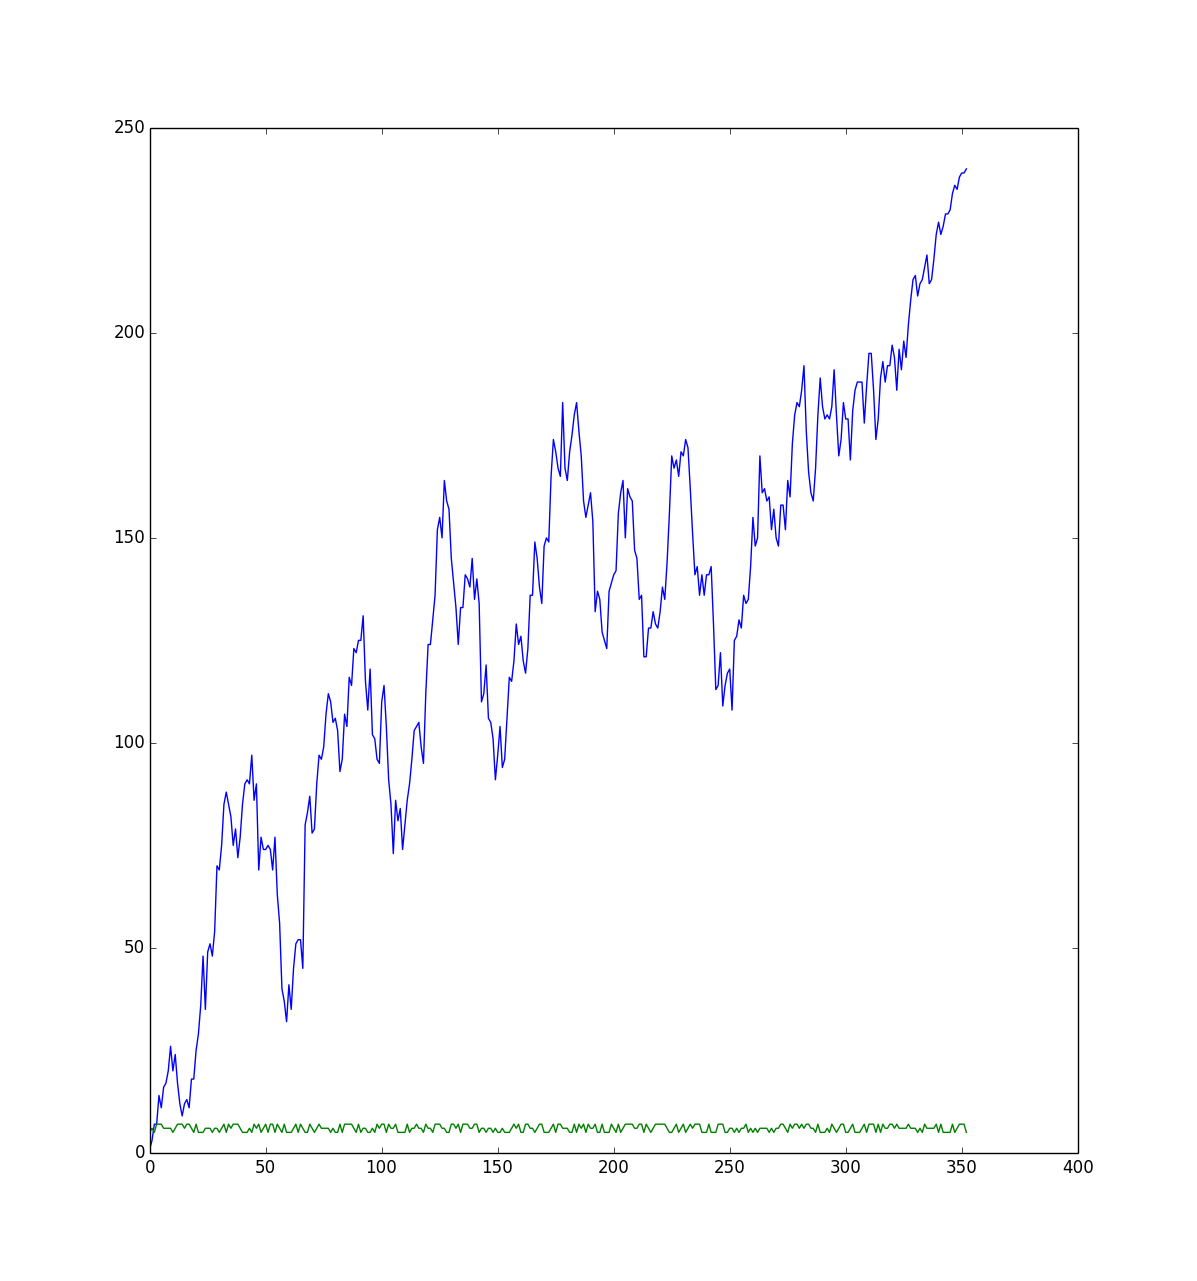
\includegraphics[scale=0.5]{slowEvolution}
\end{figure}

Alternatively, we might try to look for compelling heuristics in support of the negative answer to the research question. A closer look at any of the case simulations reveals a possible explanation: Natural selection seems to be both slow and inconsistent! The Figure \ref{slowEvolution} shows a population of size 120 undergoing selective sweep. It takes over 300 generations for the feature to spread to the entire population. It is hard to expect that such a slow process would have a big impact on something as quick as $T_{MRCA}$. Colloquially $T_{MRCA}$ is so quick that it doesn't even notice the selective process happening in the background.

Finally, one might not rule out undiscovered bugs having an effect on the result of this investigation. However, high quality and large coverage of unit-tests diminishes the risk. Additionally, it is observed that setting the relative advantage constant to very high values results in populations, where the advantageous feature spreads very quickly. Additionally, a careful inspection of the source code by another programmer than the investigator could decrease the risk even further.

\section{Topics for the future}

\begin{samepage}

An interesting observations was made during non-rigorous inspection of obtained data. Firstly, only about 4\% of advantageous features managed to spread to the entire population in the case study without dying out. It would seem wasteful for nature not to utilise so much reproductive potential. Biologists have looked at sexual selection as both stronger and more consistent form of selective pressure than natural selection \parencite{Miller14}. Could it be that switching sexual selection on could boost the spread of the feature considerably? It could make an interesting follow-up study, and another use-case for the implemented framework: to investigate relative strength of natural selection against sexual selection.

\end{samepage}

%\chapter{Glossary}
\printglossaries
\printbibliography[heading=bibintoc]
\end{document}
